% Options for packages loaded elsewhere
\PassOptionsToPackage{unicode}{hyperref}
\PassOptionsToPackage{hyphens}{url}
%
\documentclass[
]{book}
\title{Data Science für normale Anwender*innen}
\author{Prof.~Dr.~Nicolas Meseth}
\date{Aktualisiert am 18.01.2022}

\usepackage{amsmath,amssymb}
\usepackage{lmodern}
\usepackage{iftex}
\ifPDFTeX
  \usepackage[T1]{fontenc}
  \usepackage[utf8]{inputenc}
  \usepackage{textcomp} % provide euro and other symbols
\else % if luatex or xetex
  \usepackage{unicode-math}
  \defaultfontfeatures{Scale=MatchLowercase}
  \defaultfontfeatures[\rmfamily]{Ligatures=TeX,Scale=1}
\fi
% Use upquote if available, for straight quotes in verbatim environments
\IfFileExists{upquote.sty}{\usepackage{upquote}}{}
\IfFileExists{microtype.sty}{% use microtype if available
  \usepackage[]{microtype}
  \UseMicrotypeSet[protrusion]{basicmath} % disable protrusion for tt fonts
}{}
\makeatletter
\@ifundefined{KOMAClassName}{% if non-KOMA class
  \IfFileExists{parskip.sty}{%
    \usepackage{parskip}
  }{% else
    \setlength{\parindent}{0pt}
    \setlength{\parskip}{6pt plus 2pt minus 1pt}}
}{% if KOMA class
  \KOMAoptions{parskip=half}}
\makeatother
\usepackage{xcolor}
\IfFileExists{xurl.sty}{\usepackage{xurl}}{} % add URL line breaks if available
\IfFileExists{bookmark.sty}{\usepackage{bookmark}}{\usepackage{hyperref}}
\hypersetup{
  pdftitle={Data Science für normale Anwender*innen},
  pdfauthor={Prof.~Dr.~Nicolas Meseth},
  hidelinks,
  pdfcreator={LaTeX via pandoc}}
\urlstyle{same} % disable monospaced font for URLs
\usepackage{color}
\usepackage{fancyvrb}
\newcommand{\VerbBar}{|}
\newcommand{\VERB}{\Verb[commandchars=\\\{\}]}
\DefineVerbatimEnvironment{Highlighting}{Verbatim}{commandchars=\\\{\}}
% Add ',fontsize=\small' for more characters per line
\usepackage{framed}
\definecolor{shadecolor}{RGB}{248,248,248}
\newenvironment{Shaded}{\begin{snugshade}}{\end{snugshade}}
\newcommand{\AlertTok}[1]{\textcolor[rgb]{0.94,0.16,0.16}{#1}}
\newcommand{\AnnotationTok}[1]{\textcolor[rgb]{0.56,0.35,0.01}{\textbf{\textit{#1}}}}
\newcommand{\AttributeTok}[1]{\textcolor[rgb]{0.77,0.63,0.00}{#1}}
\newcommand{\BaseNTok}[1]{\textcolor[rgb]{0.00,0.00,0.81}{#1}}
\newcommand{\BuiltInTok}[1]{#1}
\newcommand{\CharTok}[1]{\textcolor[rgb]{0.31,0.60,0.02}{#1}}
\newcommand{\CommentTok}[1]{\textcolor[rgb]{0.56,0.35,0.01}{\textit{#1}}}
\newcommand{\CommentVarTok}[1]{\textcolor[rgb]{0.56,0.35,0.01}{\textbf{\textit{#1}}}}
\newcommand{\ConstantTok}[1]{\textcolor[rgb]{0.00,0.00,0.00}{#1}}
\newcommand{\ControlFlowTok}[1]{\textcolor[rgb]{0.13,0.29,0.53}{\textbf{#1}}}
\newcommand{\DataTypeTok}[1]{\textcolor[rgb]{0.13,0.29,0.53}{#1}}
\newcommand{\DecValTok}[1]{\textcolor[rgb]{0.00,0.00,0.81}{#1}}
\newcommand{\DocumentationTok}[1]{\textcolor[rgb]{0.56,0.35,0.01}{\textbf{\textit{#1}}}}
\newcommand{\ErrorTok}[1]{\textcolor[rgb]{0.64,0.00,0.00}{\textbf{#1}}}
\newcommand{\ExtensionTok}[1]{#1}
\newcommand{\FloatTok}[1]{\textcolor[rgb]{0.00,0.00,0.81}{#1}}
\newcommand{\FunctionTok}[1]{\textcolor[rgb]{0.00,0.00,0.00}{#1}}
\newcommand{\ImportTok}[1]{#1}
\newcommand{\InformationTok}[1]{\textcolor[rgb]{0.56,0.35,0.01}{\textbf{\textit{#1}}}}
\newcommand{\KeywordTok}[1]{\textcolor[rgb]{0.13,0.29,0.53}{\textbf{#1}}}
\newcommand{\NormalTok}[1]{#1}
\newcommand{\OperatorTok}[1]{\textcolor[rgb]{0.81,0.36,0.00}{\textbf{#1}}}
\newcommand{\OtherTok}[1]{\textcolor[rgb]{0.56,0.35,0.01}{#1}}
\newcommand{\PreprocessorTok}[1]{\textcolor[rgb]{0.56,0.35,0.01}{\textit{#1}}}
\newcommand{\RegionMarkerTok}[1]{#1}
\newcommand{\SpecialCharTok}[1]{\textcolor[rgb]{0.00,0.00,0.00}{#1}}
\newcommand{\SpecialStringTok}[1]{\textcolor[rgb]{0.31,0.60,0.02}{#1}}
\newcommand{\StringTok}[1]{\textcolor[rgb]{0.31,0.60,0.02}{#1}}
\newcommand{\VariableTok}[1]{\textcolor[rgb]{0.00,0.00,0.00}{#1}}
\newcommand{\VerbatimStringTok}[1]{\textcolor[rgb]{0.31,0.60,0.02}{#1}}
\newcommand{\WarningTok}[1]{\textcolor[rgb]{0.56,0.35,0.01}{\textbf{\textit{#1}}}}
\usepackage{longtable,booktabs,array}
\usepackage{calc} % for calculating minipage widths
% Correct order of tables after \paragraph or \subparagraph
\usepackage{etoolbox}
\makeatletter
\patchcmd\longtable{\par}{\if@noskipsec\mbox{}\fi\par}{}{}
\makeatother
% Allow footnotes in longtable head/foot
\IfFileExists{footnotehyper.sty}{\usepackage{footnotehyper}}{\usepackage{footnote}}
\makesavenoteenv{longtable}
\usepackage{graphicx}
\makeatletter
\def\maxwidth{\ifdim\Gin@nat@width>\linewidth\linewidth\else\Gin@nat@width\fi}
\def\maxheight{\ifdim\Gin@nat@height>\textheight\textheight\else\Gin@nat@height\fi}
\makeatother
% Scale images if necessary, so that they will not overflow the page
% margins by default, and it is still possible to overwrite the defaults
% using explicit options in \includegraphics[width, height, ...]{}
\setkeys{Gin}{width=\maxwidth,height=\maxheight,keepaspectratio}
% Set default figure placement to htbp
\makeatletter
\def\fps@figure{htbp}
\makeatother
\setlength{\emergencystretch}{3em} % prevent overfull lines
\providecommand{\tightlist}{%
  \setlength{\itemsep}{0pt}\setlength{\parskip}{0pt}}
\setcounter{secnumdepth}{5}
\usepackage{booktabs}
\ifLuaTeX
  \usepackage{selnolig}  % disable illegal ligatures
\fi
\usepackage[]{natbib}
\bibliographystyle{plainnat}
\nocite{wickham_r_2016}

\begin{document}
\maketitle

{
\setcounter{tocdepth}{1}
\tableofcontents
}
\hypertarget{uxfcbersicht}{%
\chapter*{Übersicht}\label{uxfcbersicht}}
\addcontentsline{toc}{chapter}{Übersicht}

\hypertarget{zielgruppe}{%
\section*{Zielgruppe}\label{zielgruppe}}
\addcontentsline{toc}{section}{Zielgruppe}

Dieses Buch gibt eine Einführung in wichtige Themen bei der Arbeit mit Daten. Wie der Titel schon ahnen lässt, adressiert dieses Buch \emph{normale} Anwender*innen. Damit meine ich Personen, die in ihrem beruflichen (oder privaten) Alltag von Kenntnissen in der Analyse von Daten (über Excel hinaus) profitieren, diese aber nicht deren Haupttätigkeit ist.

In genau diese Zielgruppe fallen mehr als 95\% der Studierenden, die an der \href{https://hs-osnabrueck.de}{Hochschule Osnabrück} in jedem Semester an meinen Vorlesungen und Seminaren teilnehmen. Sie studieren einen Studiengang aus der Fachrichtung Agrar- oder Lebensmittelwirtschaft und haben in meinen Veranstaltungen die Möglichkeit, zusätzliche Kompetenzen zu digitalen Themen zu entwickeln. Sie arbeiten später aber nicht in IT-Berufen oder als Data Scientist. Sie sind aber dafür gerüstet, mit diesen Abteilungen (IT / Data Scientists) besser zusammenzuarbeiten und viele Dinge können sie auch in Eigenregie umsetzen. Dazu zählen beispielsweise Datenanalysen und -visualisierungen mit R.

\hypertarget{didaktisches-konzept}{%
\section*{Didaktisches Konzept}\label{didaktisches-konzept}}
\addcontentsline{toc}{section}{Didaktisches Konzept}

Das Buch ist in fortlaufend nummerierte Kapitel gegliedert. Man folgt meinem didaktischen Konzept, wenn man diese Reihenfolge einhält. Dieses Konzept beruht darauf, sich zuerst \emph{hands-on} mit einem Thema auseinanderzusetzen, bevor die relevanen theoretischen Hintergründe eingeführt werden. Meiner Erfahrung nach sind theoretische Hintergründe einfacher zu verstehen, wenn das Subjekt der Betrachtung bereits in den Händen war. Der Kontext ist präsent und man weiß bei fachlichen Begriffen sofort die richtige Assoziation herzustellen.

Ein zweiter wichtiger Gedanke beim didaktischen Aufbau des Buches ist die Verwendung von Beispielen aus der Praxis. Dazu zählen insbesodere Datensätze und Fragen an diese Daten. Jedes Kapitel beinhaltet Beispiele und Übungen mit Bezug zu Daten aus der Praxis. Die Anwendungsfälle hinter den Daten reichen von Onlineumfragen aus der Markforschung über Daten aus Laborexperimenten bis hin zu Datensätzen aus sozialen Medien wie Twitter. Alle Datensätze, die in diesem Buch verwendet werden, sind im Kapitel \protect\hyperlink{datensaetze}{Datensätze} gelistet.

Nicht immer ist es sinnvoll, ein neues Konzept anhand eines Datensatzes aus der Praxis einzuführen. In diesem Fall greife ich auf synthetische Datensätze zurück, um die Idee oder das Konzept möglichst plastisch darstellen zu können. Die Anwendung des eingeführten Konzepts auf Datensätze aus der Praxis erfolgt dann anschließend. Es sollte in diesem Buch kein Konzept eingeführt werden, das nicht in der Praxis relevant ist.

Das Buch kann selbstverständlich abseits des didaktischen Konzepts verwendet werden. Ich habe beim Verfassen darauf geachtet, das jedes Kapitel in sich geschlossen ist und einzeln gelesen und bearbeitet werden kann. Das gilt auch für die Übungen für die Anwendung mit R.

\hypertarget{part-erste-schritte-mit-r}{%
\part*{Erste Schritte mit R}\label{part-erste-schritte-mit-r}}
\addcontentsline{toc}{part}{Erste Schritte mit R}

\hypertarget{die-arbeitsumgebung}{%
\chapter{Die Arbeitsumgebung}\label{die-arbeitsumgebung}}

\hypertarget{tldr}{%
\section*{TL;DR}\label{tldr}}

\begin{itemize}
\tightlist
\item
  Für die Arbeit mit R benötigen wir eine Installation von R auf unserem Computer.
\item
  R ist für alle Betriebssysteme \href{https://cran.r-project.org/}{verfügbar}.
\item
  Mit R bekommen wir auch eine einfache grafische Benutzeroberfläche (RGui) mitgeliefert. Diese bietet aber wenig Funktionen.
\item
  Mit dem kostenlosen \href{https://www.rstudio.com/}{RStudio} bekommen wir eine vollwertige integrierte Entwicklungsumgebung (IDE) für die Arbeit R.
\end{itemize}

\hypertarget{r-installieren}{%
\section{R installieren}\label{r-installieren}}

R ist eine Open-Source-Software und für alle gängigen Betriebssysteme verfügbar. Ladet euch zunächst die neueste Version von R für euer Betriebssystem herunter und installiert es anschließend:

\begin{itemize}
\tightlist
\item
  \href{https://cran.r-project.org/bin/windows/base/}{R für Windows}
\item
  \href{https://cran.r-project.org/bin/macosx/}{R für macOS}
\item
  \href{https://cran.r-project.org/bin/linux/}{R für Linux}
\end{itemize}

Neben der Sprache und dem Interpreter für R erhaltet ihr mit der Installation auch eine rudimentäre grafische Oberfläche mit dem Namen \emph{RGui} (GUI = Graphical User Interface). Diese besteht aus einer einfachen Konsole, über die ihr R-Befehle eingeben und ausführen könnt.

\begin{figure}
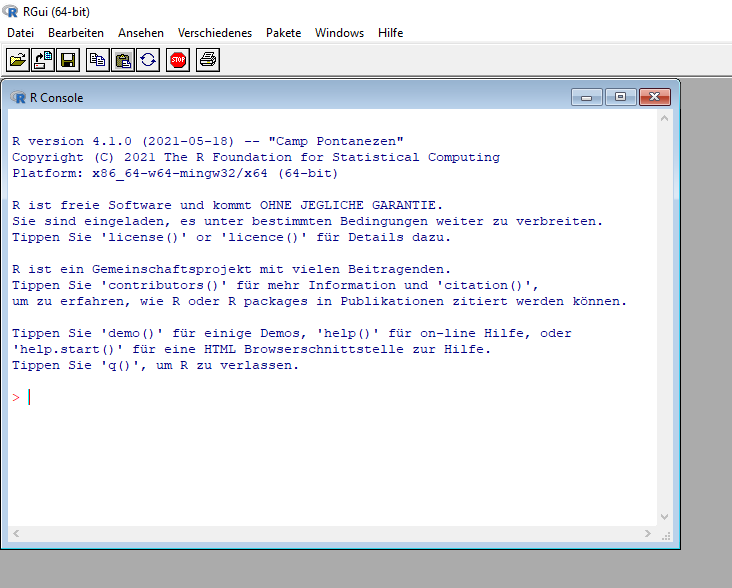
\includegraphics[width=1\linewidth]{fig/screenshot_r_console} \caption{Die RGui bietet einen rudimentären Editor für R-Befehle.}\label{fig:screenshot-r-console}
\end{figure}

Erweiterte Funktionen wie Autovervollständigung beim Schreiben von R-Code, ein integrierter Debugger für die Fehlersuche, eine Echtzeit-Vorschau für R-Markdown und viele andere Features mehr bietet dieses einfache Tool nicht. Deshalb verwenden wir für die Arbeit mit R nicht die RGui, sondern das ebenfalls kostenlos nutzbare \href{https://www.rstudio.com/products/rstudio/}{RStudio}.

\hypertarget{rstudio-installieren}{%
\section{RStudio installieren}\label{rstudio-installieren}}

Das \href{https://www.rstudio.com/}{RStudio} ist das Standardwerkzeug für die Arbeit mit R und bietet dafür viele nützliche Funktionen. Das RStudio ist ein sogenanntes \textbf{Integrated Development Environment (IDE)} für R. Einen schnellen Überblick über die grafische Benutzeroberfläche findet ihr in dem offiziellen \href{https://raw.githubusercontent.com/rstudio/cheatsheets/main/rstudio-ide.pdf}{RStudio Cheatsheet}.

Klickt auf den Link unten und wählt RStudio für euer Betriebssystem aus. Installiert RStudio und öffnet es:

\begin{itemize}
\tightlist
\item
  \href{https://www.rstudio.com/products/rstudio/download/\#download}{RStudio herunterladen}
\end{itemize}

Nach dem Öffnen seht ihr die Oberfläche des RStudio, die wie auf dem Screenshot unten aussieht:

\begin{figure}
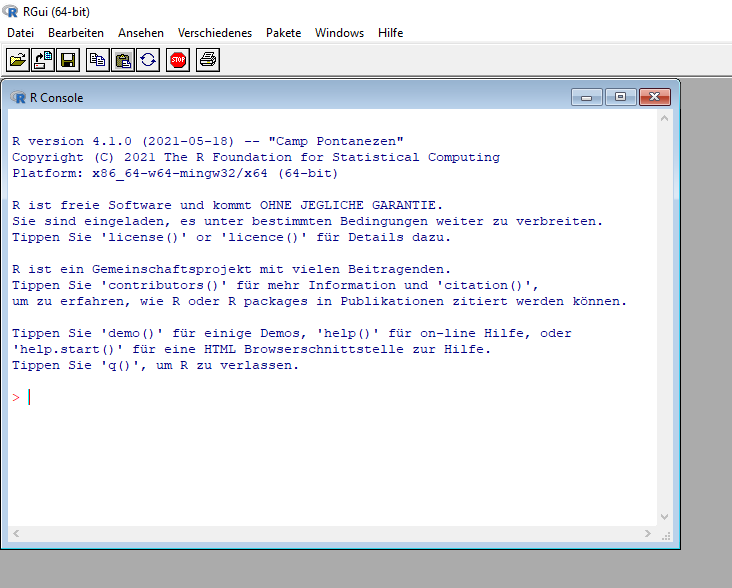
\includegraphics[width=1\linewidth]{fig/screenshot_r_console} \caption{Das RStudio ist in vier Bereiche eingeteilt.}\label{fig:screenshot-rstudio}
\end{figure}

\hypertarget{uxfcberblick-uxfcber-rstudio}{%
\section{Überblick über RStudio}\label{uxfcberblick-uxfcber-rstudio}}

Das Werkzeug besteht in der Standardansicht aus vier Bereichen (s. Screenshot oben):

\hypertarget{der-skripteditor}{%
\subsection{Der Skripteditor}\label{der-skripteditor}}

Der wichtigste Bereich ist der Skripteditor. Hier schreiben wir unseren R-Code und speichern ihn in Dateien auf unserem Computer. Dabei unterstützt uns RStudio mit vielen nützlichen Funktionen.

Wir können in RStudio unterschiedliche Arten von Dateien verwenden, um unsere Skripte zu speichern. Die einfachste Art sind sogenannte \textbf{R-Skripte} mit der Dateiendung \texttt{.R}. Wenn wir nicht nur R-Code, sondern auch Visualisierungen und formatierten Text in einem Dokument verwenden und anzeigen wollen, bietet sich die Verwendung eines \textbf{R-Notebooks} an. Eine R-Notebook-Datei endet auf \texttt{.Rmd} (R-Markdown) und wir können neben R-Code auch Markdown verwenden. Über Markdown lernen wir zu einem späteren Zeitpunkt mehr.

\hypertarget{informationen-zur-aktuellen-r-umgebung}{%
\subsection{Informationen zur aktuellen R-Umgebung}\label{informationen-zur-aktuellen-r-umgebung}}

R erstellt für die Ausführung von Skripten eine sogenannte Session. In einer Session werden alle Objekte, wie die momentan verwendeten Daten, eigene Variablen oder Funktionen, im Arbeitsspeicher des lokalen Rechners gespeichert. In dem zweiten Fenster können im Tab \emph{Environment} alle Objekte, die es in der aktuellen Session gibt, in der Übersicht und im Detail betrachtet werden. Der \emph{History} Tab enthält eine Liste aller ausgeführten Befehle in der aktuellen Session. Daneben gibt es noch den \emph{Connections} Tab für die Verbindung zu unterschiedlichen Datenquellen, wie Datenbanken oder Webservices, sowie den \emph{Tutorial} Tab, in dem direkt in RStudio unterschiedliche Anleitungen angezeigt werden können.

\{\% hint style=``info'' \%\}
Für die Anzeige von Tutorials direkt in RStudio muss das Paket \texttt{learnr} installiert werden. Ihr müsst der Installation einmalig zustimmen und das Paket installieren.
\{\% endhint \%\}

\hypertarget{konsole-und-terminal}{%
\subsection{Konsole und Terminal}\label{konsole-und-terminal}}

Die Konsole ermöglicht, R-Befehle einzugeben und mit der Taste Enter auszuführen. Die Konsole in RStudio ist fast identisch zu der RGui. Für das schnelle Ausprobieren von Befehlen kann die Konsole nützlich sein. Für die strukturierte Arbeit mit den Daten sollten wir aber den Skripteditor verwenden, weil wir dort unsere Arbeit speichern und mit Kommentaren versehen können.

\hypertarget{dateien-vorschau-und-plots}{%
\subsection{Dateien, Vorschau und Plots}\label{dateien-vorschau-und-plots}}

In diesem Bereich werden Vorschauen unterschiedlicher Artefakte angezeigt. Dazu gehören gerenderte R-Notebooks, Markdown, aber auch Visualisierungen. In diesem Bereich gibt es auch einen rudimentären Datei-Explorer, um Dateien wie Skripte oder Datendateien zu finden und von dort zu öffnen.

\hypertarget{einen-datensatz-laden}{%
\chapter{Einen Datensatz laden}\label{einen-datensatz-laden}}

Nachdem die Arbeitsumgebung eingerichtet ist, können wir mit den ersten Schritten in R beginnen. Wir steigen direkt ein und lernen, wie wir mit Daten in R arbeiten.

\hypertarget{tldr-1}{%
\section*{TL;DR}\label{tldr-1}}

\begin{itemize}
\tightlist
\item
  R bietet verschiedene Möglichkeiten, um mit Daten zu arbeiten.
\item
  Für strukturierte Daten in Tabellenform (Zeilen und Spalten) verwenden wir in R den \protect\hyperlink{der-dataframe}{Dataframe}.
\item
  Eine modernere Version des klassischen Dataframe ist das \protect\hyperlink{tibbles}{Tibble} aus dem \protect\hyperlink{das-tidyverse}{Tidyverse}.
\end{itemize}

\hypertarget{tabellarische-daten-in-r}{%
\section{Tabellarische Daten in R}\label{tabellarische-daten-in-r}}

\hypertarget{der-dataframe}{%
\subsection{Der Dataframe}\label{der-dataframe}}

In R gibt es verschiedene Strukturen für die Speicherung von Daten. Darunter sind beispielsweise Vektoren, Listen oder Matritzen. Um tabellarische Daten abzubilden, die in Spalten und Zeilen organisiert sind, verwenden wir in R den sogenannten \textbf{Dataframe}.

\hypertarget{tibbles}{%
\subsection{Tibbles}\label{tibbles}}

Der Tibble ist eine Weiterentwicklung des klassischen Dataframe in R. Tibbles werden im Tidyverse standardmäßig verwendet und mit dem Paket \texttt{tibble} eingeführt.

\hypertarget{das-csv-format}{%
\section{Das CSV-Format}\label{das-csv-format}}

In den meisten Fällen erzeugen wir einen Dataframe oder Tibble, indem wir einen Datensatz aus einer Datenquelle laden. Häufig ist die Quelle eine einfache Texdatei, in der Daten zeilenweise gespeichert sind und jede Zeile aus mehreren einzelnen Werten besteht, die durch ein bestimmtes \textbf{Trennzeichen} voneinander getrennt sind. Wenn die Werte mit einem Komma voneinander getrennt sind, nennt man das Format \textbf{CSV}. CSV steht für \textbf{Comma Separated Values}, was auf Deutsch so viel wie \emph{Durch Kommata getrennte Werte} bedeutet.

Unten seht ihr ein Beispiel für Daten im CSV-Format.

\begin{verbatim}
id,firstname,lastname
1,Boris,Becker
2,Steffi,Graf
3,Rafael, Nadal
\end{verbatim}

Die erste Zeile nennen wir auch Kopfzeile oder \emph{Header}. Sie beinhaltet die Spaltennamen. Jede nachfolgende Zeile stellt einen Datensatz oder \emph{Record} dar. Dabei müssen die Werte in jeder Zeile mit Komma getrennt in der selben Reihenfolge wie im Header aufgeführt werden. Nur so ist eindeutig erkennbar, welcher Wert zu welcher Spalte gehört.

Manchmal fehlen Werte für eine bestimmte Spalte. In diesem Fall werden einfach zwei (oder mehrere) Kommata hintereinander gesetzt.

\begin{verbatim}
id,firstname,lastname,height,weight,gender
1,Boris,Becker,,,male
2,Steffi,Graf,175,64,female
3,Rafael,Nadal,185,,male
\end{verbatim}

\hypertarget{csv-daten-laden}{%
\section{CSV-Daten laden}\label{csv-daten-laden}}

\begin{Shaded}
\begin{Highlighting}[]
\FunctionTok{library}\NormalTok{(readr)}
\NormalTok{food\_production }\OtherTok{\textless{}{-}} \FunctionTok{read\_csv}\NormalTok{(}\StringTok{"food\_production.csv"}\NormalTok{)}
\end{Highlighting}
\end{Shaded}

\hypertarget{einen-datensatz-erkunden}{%
\chapter{Einen Datensatz erkunden}\label{einen-datensatz-erkunden}}

\hypertarget{tldr-2}{%
\section*{TL;DR}\label{tldr-2}}

\begin{itemize}
\tightlist
\item
  In RStudio können wir mit \texttt{view} den gesamten Dataframe oder Tibble \protect\hyperlink{alle-daten-anzeigen}{im Skripteditor anzeigen}.
\item
  Die \protect\hyperlink{spaltennamen-ermitteln}{Spaltennamen} eines Tibble erhalten wir mit \texttt{colnames}.
\item
  Mit \texttt{glimpse} können wir einen Überblick der Spalten und enthaltenen Werte anzeigen.
\item
  Mit \texttt{ncol} und \texttt{nrow} erhalten wir die \protect\hyperlink{anzahl-spalten-zeilen}{Anzahl Spalten und Zeilen} eines Tibbles. Das Gleiche bekommen wir in einem Schwung mit der Funktion \texttt{dim}.
\item
  Einen schnellen \protect\hyperlink{wertebereich-nominalskaliert}{Überblick über eine nominalskalierte Spalte und deren Werte} bekommen wir mit \texttt{distinct} (eindeutige Werte) oder \texttt{count} (zusätzlich die Häufigkeiten).
\item
  Für \protect\hyperlink{wertebereich-intervallskaliert}{intervallskalierte Werte} können wir besser mit \texttt{min} und \texttt{max} die Spannweite ermitteln oder mit einem \protect\hyperlink{wertebereich-intervallskaliert-histogramm}{Histogramm die Verteilung der Werte visualisieren}.
\item
  Mit \texttt{is.na} können wir prüfen, ob ein Wert NA ist (nicht vorhanden) und so auch die Anzahl fehlender Werte ermitteln.
\item
  Mit der \texttt{summary} Funktion erzeugen wir eine Übersicht wichtiger statistischer Kennzahlen für eine Spalte.
\item
  Mit \texttt{head} und \texttt{tail} erhalten wir die ersten oder letzten 10 Zeilen eines Tibble. Mit dem einzigen Parameter der Funktion können wir auch eine andere Anzahl zurückgeben.
\end{itemize}

\hypertarget{alle-daten-anzeigen}{%
\section{Alle Daten anzeigen}\label{alle-daten-anzeigen}}

Oft ist es hilfreich, einen schnellen Blick in einen Datensatz zu werfen, um beispielsweise die Werte einer Spalte zu überprüfen. Dafür können wir in RStudio die Funktion \texttt{view()} verwenden. Der Funktion übergeben wir den Tibble \texttt{pokemon}:

\begin{Shaded}
\begin{Highlighting}[]
\FunctionTok{view}\NormalTok{(pokemon)}
\end{Highlighting}
\end{Shaded}

Mit ⌨ Strg + Enter oder über den Button „Run`` in der rechten oberen Ecke des Skriptfensters führen wir die Zeile aus. Es öffnet sich ein neuer Tab mit einer tabellarischen Ansicht der Daten.

\begin{figure}
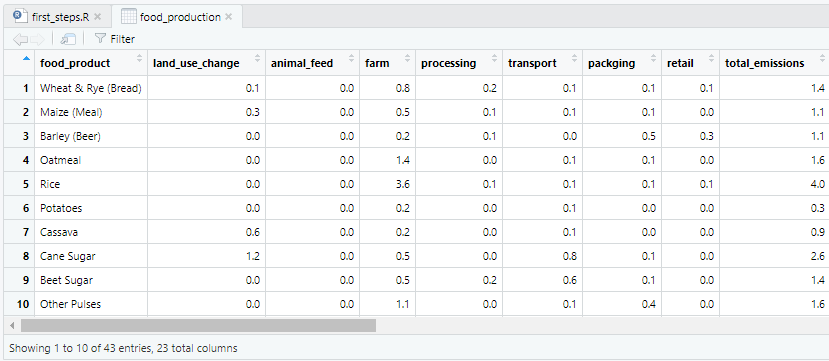
\includegraphics[width=1\linewidth]{fig/view_result_rstudio} \caption{Die Anzeige eines Tibbles in RStudio mit `view`.}\label{fig:fig-view-rstudio}
\end{figure}

\hypertarget{spaltennamen-ermitteln}{%
\section{Spaltenamen ermitteln}\label{spaltennamen-ermitteln}}

Um mit einem Datensatz arbeiten zu können, benötigen wir eine Übersicht über seine Spalten. Diese liefert und die Funktion \texttt{colnames}:

\begin{Shaded}
\begin{Highlighting}[]
\NormalTok{pokemon }\SpecialCharTok{\%\textgreater{}\%}
  \FunctionTok{colnames}\NormalTok{()}
\end{Highlighting}
\end{Shaded}

\begin{verbatim}
##  [1] "abilities"         "against_bug"       "against_dark"     
##  [4] "against_dragon"    "against_electric"  "against_fairy"    
##  [7] "against_fight"     "against_fire"      "against_flying"   
## [10] "against_ghost"     "against_grass"     "against_ground"   
## [13] "against_ice"       "against_normal"    "against_poison"   
## [16] "against_psychic"   "against_rock"      "against_steel"    
## [19] "against_water"     "attack"            "base_egg_steps"   
## [22] "base_happiness"    "base_total"        "capture_rate"     
## [25] "classfication"     "defense"           "experience_growth"
## [28] "height_m"          "hp"                "japanese_name"    
## [31] "name"              "percentage_male"   "pokedex_number"   
## [34] "sp_attack"         "sp_defense"        "speed"            
## [37] "type1"             "type2"             "weight_kg"        
## [40] "generation"        "is_legendary"
\end{verbatim}

Auf diese Information greifen wir zurück, wenn wir später Analysen mit dem Datensatz durchführen oder bestimmte Spalten genauer untersuchen wollen.

\hypertarget{schnelle-uxfcbersicht-der-spalten-datentypen-und-werte}{%
\section{Schnelle Übersicht der Spalten, Datentypen und Werte}\label{schnelle-uxfcbersicht-der-spalten-datentypen-und-werte}}

\begin{Shaded}
\begin{Highlighting}[]
\FunctionTok{glimpse}\NormalTok{(pokemon)}
\end{Highlighting}
\end{Shaded}

\begin{verbatim}
## Rows: 801
## Columns: 41
## $ abilities         <chr> "['Overgrow', 'Chlorophyll']", "['Overgrow', 'Chloro~
## $ against_bug       <dbl> 1.00, 1.00, 1.00, 0.50, 0.50, 0.25, 1.00, 1.00, 1.00~
## $ against_dark      <dbl> 1, 1, 1, 1, 1, 1, 1, 1, 1, 1, 1, 1, 1, 1, 1, 1, 1, 1~
## $ against_dragon    <dbl> 1, 1, 1, 1, 1, 1, 1, 1, 1, 1, 1, 1, 1, 1, 1, 1, 1, 1~
## $ against_electric  <dbl> 0.5, 0.5, 0.5, 1.0, 1.0, 2.0, 2.0, 2.0, 2.0, 1.0, 1.~
## $ against_fairy     <dbl> 0.5, 0.5, 0.5, 0.5, 0.5, 0.5, 1.0, 1.0, 1.0, 1.0, 1.~
...
\end{verbatim}

\hypertarget{anzahl-spalten-zeilen}{%
\section{Anzahl Spalten und Zeilen ermitteln}\label{anzahl-spalten-zeilen}}

Einfache Informationen wie die Anzahl Spalten und Zeilen ermitteln wir mit den Funktionen \texttt{ncol}, \texttt{nrow} oder \texttt{dim}.

\begin{Shaded}
\begin{Highlighting}[]
\NormalTok{pokemon }\SpecialCharTok{\%\textgreater{}\%}
  \FunctionTok{ncol}\NormalTok{()}
\end{Highlighting}
\end{Shaded}

\begin{verbatim}
## [1] 41
\end{verbatim}

\begin{Shaded}
\begin{Highlighting}[]
\NormalTok{pokemon }\SpecialCharTok{\%\textgreater{}\%}
  \FunctionTok{nrow}\NormalTok{()}
\end{Highlighting}
\end{Shaded}

\begin{verbatim}
## [1] 801
\end{verbatim}

Wenn wir beide Werte in einer Ausgabe haben wollen können wir \texttt{dim} verwenden:

\begin{Shaded}
\begin{Highlighting}[]
\NormalTok{pokemon }\SpecialCharTok{\%\textgreater{}\%}
  \FunctionTok{dim}\NormalTok{()}
\end{Highlighting}
\end{Shaded}

\begin{verbatim}
## [1] 801  41
\end{verbatim}

\texttt{dim} gibt einen Vektor mit zwei Werten zurück. Der erste Wert steht für die Anzahl Zeilen, der zweite für die Anzahl Spalten. Wir können mit der Angabe der Position in eckigen Klammern auf jeden Wert einzeln zugreifen:

\begin{Shaded}
\begin{Highlighting}[]
\NormalTok{dimensions }\OtherTok{\textless{}{-}}\NormalTok{ pokemon }\SpecialCharTok{\%\textgreater{}\%} \FunctionTok{dim}\NormalTok{()}

\CommentTok{\# Anzahl Zeilen}
\NormalTok{dimensions[}\DecValTok{1}\NormalTok{]}
\end{Highlighting}
\end{Shaded}

\begin{verbatim}
## [1] 801
\end{verbatim}

Und auf die Spalten:

\begin{Shaded}
\begin{Highlighting}[]
\CommentTok{\# Anzahl Spalten}
\NormalTok{dimensions[}\DecValTok{2}\NormalTok{]}
\end{Highlighting}
\end{Shaded}

\begin{verbatim}
## [1] 41
\end{verbatim}

\hypertarget{wertebereich-von-spalten-bestimmen}{%
\section{Wertebereich von Spalten bestimmen}\label{wertebereich-von-spalten-bestimmen}}

\hypertarget{wertebereich-nominalskaliert}{%
\subsection{Nominalskalierte Spalten}\label{wertebereich-nominalskaliert}}

\hypertarget{eindeutige-werte-mit-distinct}{%
\subsubsection{\texorpdfstring{Eindeutige Werte mit \texttt{distinct}}{Eindeutige Werte mit distinct}}\label{eindeutige-werte-mit-distinct}}

Für nominalskalierte Spalten kann es interessant sein, alle Werte und eventuell deren Häufigkeit anzuzeigen. Die eindeutigen Werte bekommen wir mit der \texttt{distinct} Funktion:

\begin{Shaded}
\begin{Highlighting}[]
\NormalTok{pokemon }\SpecialCharTok{\%\textgreater{}\%}
  \FunctionTok{distinct}\NormalTok{(type2)}
\end{Highlighting}
\end{Shaded}

\begin{verbatim}
## # A tibble: 19 x 1
##    type2   
##    <chr>   
##  1 poison  
##  2 <NA>    
##  3 flying  
##  4 dark    
##  5 electric
...
\end{verbatim}

\hypertarget{eindeutige-werte-und-deren-huxe4ufigkeiten}{%
\subsubsection{Eindeutige Werte und deren Häufigkeiten}\label{eindeutige-werte-und-deren-huxe4ufigkeiten}}

Wenn wir zusätzlich noch die Häufigkeiten ermitteln wollen, können wir die Funktion \texttt{count} verwenden und als Parameter den Spaltennamen übergeben:

\begin{Shaded}
\begin{Highlighting}[]
\NormalTok{pokemon }\SpecialCharTok{\%\textgreater{}\%} 
  \FunctionTok{count}\NormalTok{(type1)}
\end{Highlighting}
\end{Shaded}

\begin{verbatim}
## # A tibble: 18 x 2
##    type1        n
##    <chr>    <int>
##  1 bug         72
##  2 dark        29
##  3 dragon      27
##  4 electric    39
##  5 fairy       18
...
\end{verbatim}

Meist es nützlich, direkt nach Häufigkeiten zu sortieren:

\begin{Shaded}
\begin{Highlighting}[]
\NormalTok{pokemon }\SpecialCharTok{\%\textgreater{}\%} 
  \FunctionTok{count}\NormalTok{(type1, }\AttributeTok{sort =} \ConstantTok{TRUE}\NormalTok{)}
\end{Highlighting}
\end{Shaded}

\begin{verbatim}
## # A tibble: 18 x 2
##    type1        n
##    <chr>    <int>
##  1 water      114
##  2 normal     105
##  3 grass       78
##  4 bug         72
##  5 psychic     53
...
\end{verbatim}

\hypertarget{wertebereich-intervallskaliert}{%
\subsection{Intervallskalierte Spalten}\label{wertebereich-intervallskaliert}}

Für intervallskalierte Spalten, also Spalten mit Zahlenwerten, eignen sich die Funktionen \texttt{distinct} und \texttt{count} nur bedingt. Oft sind es zu viele unterschiedliche Werte und das reine Zählen bringt nicht viel Aufschluss. Wenn wir distinct auf die Spalte \texttt{weight\_kg} anwenden, erhalten wir zum Beispiel 422 unterschiedliche Werte:

\begin{Shaded}
\begin{Highlighting}[]
\NormalTok{pokemon }\SpecialCharTok{\%\textgreater{}\%}
  \FunctionTok{distinct}\NormalTok{(weight\_kg)}
\end{Highlighting}
\end{Shaded}

\begin{verbatim}
## # A tibble: 422 x 1
##    weight_kg
##        <dbl>
##  1       6.9
##  2      13  
##  3     100  
##  4       8.5
##  5      19  
##  6      90.5
##  7       9  
##  8      22.5
##  9      85.5
## 10       2.9
## # ... with 412 more rows
\end{verbatim}

In diesem Fall ist es sinnvoller, den kleinsten und größten Wert zu kennen, um die \textbf{Spannweite} der Spalte zu ermitteln. Interessant wäre auch die Verteilung der Werte, etwa in Form eines Histogramm.

\hypertarget{gruxf6uxdfter-und-kleinster-wert}{%
\subsubsection{Größter und kleinster Wert}\label{gruxf6uxdfter-und-kleinster-wert}}

Den größten oder kleinsten Wert können wir mit \texttt{max} und \texttt{min} ermitteln:

\begin{Shaded}
\begin{Highlighting}[]
\NormalTok{pokemon }\SpecialCharTok{\%\textgreater{}\%}
  \FunctionTok{select}\NormalTok{(weight\_kg) }\SpecialCharTok{\%\textgreater{}\%}
  \FunctionTok{max}\NormalTok{(}\AttributeTok{na.rm =} \ConstantTok{TRUE}\NormalTok{)}
\end{Highlighting}
\end{Shaded}

\begin{verbatim}
## [1] 999.9
\end{verbatim}

\begin{Shaded}
\begin{Highlighting}[]
\NormalTok{pokemon }\SpecialCharTok{\%\textgreater{}\%}
  \FunctionTok{select}\NormalTok{(weight\_kg) }\SpecialCharTok{\%\textgreater{}\%}
  \FunctionTok{min}\NormalTok{(}\AttributeTok{na.rm =} \ConstantTok{TRUE}\NormalTok{)}
\end{Highlighting}
\end{Shaded}

\begin{verbatim}
## [1] 0.1
\end{verbatim}

Wir wissen also, dass die Werte sich zwischen 0,1 und 999,9 bewegen. Wie aber sind die Werte dazwischen verteilt?

\hypertarget{wertebereich-intervallskaliert-histogramm}{%
\subsubsection{Verteilung der Werte als Histogramm}\label{wertebereich-intervallskaliert-histogramm}}

Um die Verteilung der Werte innerhalb der Spalte \texttt{weight\_kg} sinnvoll zu ermitteln müssen wir an dieser Stelle einen Exkurs in die Visualisierung von Daten machen:

\begin{Shaded}
\begin{Highlighting}[]
\NormalTok{pokemon }\SpecialCharTok{\%\textgreater{}\%}
  \FunctionTok{select}\NormalTok{(weight\_kg) }\SpecialCharTok{\%\textgreater{}\%}
  \FunctionTok{filter}\NormalTok{(}\SpecialCharTok{!}\FunctionTok{is.na}\NormalTok{(weight\_kg)) }\SpecialCharTok{\%\textgreater{}\%}
  \FunctionTok{ggplot}\NormalTok{() }\SpecialCharTok{+}
  \FunctionTok{aes}\NormalTok{(}\AttributeTok{x =}\NormalTok{ weight\_kg) }\SpecialCharTok{+}
  \FunctionTok{geom\_histogram}\NormalTok{(}\AttributeTok{bins =} \DecValTok{50}\NormalTok{)}
\end{Highlighting}
\end{Shaded}

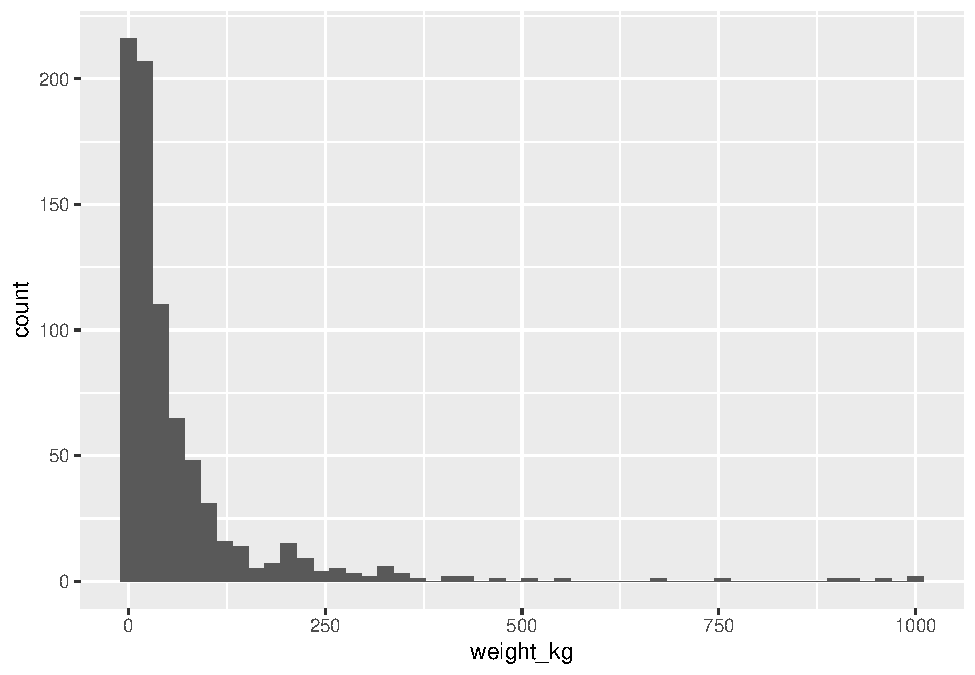
\includegraphics{_main_files/figure-latex/unnamed-chunk-16-1.pdf}

Das Historgramm zeigt uns, dass der größte Teil der Daten im kleineren Bereich liegt und nur wenige Ausnahmen große Werte jenseits der 300 aufweisen.

\hypertarget{anzahl-fehlender-werte}{%
\subsubsection{Anzahl fehlender Werte}\label{anzahl-fehlender-werte}}

Die Anzahl fehlender Werte, die in R als \texttt{NA} dargestellt werden, ist ein wichtiges Merkmal für die Qualität der Daten einer Spalte. Um diese Zahl zu ermitteln filtern wir die Daten mit der Funktion \texttt{is.na} und zählen anschließend die übrig gebliebenen Werte:

\begin{Shaded}
\begin{Highlighting}[]
\NormalTok{pokemon }\SpecialCharTok{\%\textgreater{}\%}
  \FunctionTok{select}\NormalTok{(weight\_kg) }\SpecialCharTok{\%\textgreater{}\%}
  \FunctionTok{filter}\NormalTok{(}\FunctionTok{is.na}\NormalTok{(weight\_kg)) }\SpecialCharTok{\%\textgreater{}\%}
  \FunctionTok{count}\NormalTok{()}
\end{Highlighting}
\end{Shaded}

\begin{verbatim}
## # A tibble: 1 x 1
##       n
##   <int>
## 1    20
\end{verbatim}

Insgesamt haben somit 20 Pokémon keine Gewichtsangabe.

\hypertarget{zusammenfassung-einer-spalte-ausgeben}{%
\subsubsection{Zusammenfassung einer Spalte ausgeben}\label{zusammenfassung-einer-spalte-ausgeben}}

Um gleich mehrer statistische Größen zu berechnen und auszugeben können wir die Funktion \texttt{summary} verwenden:

\begin{Shaded}
\begin{Highlighting}[]
\NormalTok{pokemon }\SpecialCharTok{\%\textgreater{}\%}
  \FunctionTok{select}\NormalTok{(weight\_kg) }\SpecialCharTok{\%\textgreater{}\%}
  \FunctionTok{summary}\NormalTok{()}
\end{Highlighting}
\end{Shaded}

\begin{verbatim}
##    weight_kg     
##  Min.   :  0.10  
##  1st Qu.:  9.00  
##  Median : 27.30  
##  Mean   : 61.38  
##  3rd Qu.: 64.80  
##  Max.   :999.90  
##  NA's   :20
\end{verbatim}

\hypertarget{erste-oder-letzte-zeilen-anzeigen}{%
\section{Erste oder letzte Zeilen anzeigen}\label{erste-oder-letzte-zeilen-anzeigen}}

Die Funktion \texttt{head} gibt die ersten 10 Zeilen eines Tibbles zurück:

\begin{Shaded}
\begin{Highlighting}[]
\NormalTok{pokemon }\SpecialCharTok{\%\textgreater{}\%}
  \FunctionTok{head}\NormalTok{()}
\end{Highlighting}
\end{Shaded}

\begin{verbatim}
## # A tibble: 6 x 41
##   abilities             against_bug against_dark against_dragon against_electric
##   <chr>                       <dbl>        <dbl>          <dbl>            <dbl>
## 1 ['Overgrow', 'Chloro~        1               1              1              0.5
## 2 ['Overgrow', 'Chloro~        1               1              1              0.5
## 3 ['Overgrow', 'Chloro~        1               1              1              0.5
## 4 ['Blaze', 'Solar Pow~        0.5             1              1              1  
## 5 ['Blaze', 'Solar Pow~        0.5             1              1              1  
## 6 ['Blaze', 'Solar Pow~        0.25            1              1              2  
## # ... with 36 more variables: against_fairy <dbl>, against_fight <dbl>,
## #   against_fire <dbl>, against_flying <dbl>, against_ghost <dbl>,
## #   against_grass <dbl>, against_ground <dbl>, against_ice <dbl>,
## #   against_normal <dbl>, against_poison <dbl>, against_psychic <dbl>,
## #   against_rock <dbl>, against_steel <dbl>, against_water <dbl>, attack <dbl>,
## #   base_egg_steps <dbl>, base_happiness <dbl>, base_total <dbl>,
## #   capture_rate <chr>, classfication <chr>, defense <dbl>, ...
\end{verbatim}

Über den Parameter der Funktion können wir die Anzahl der Zeilen verändern, um etwa nur die erste Zeile zu erhalten:

\begin{Shaded}
\begin{Highlighting}[]
\NormalTok{pokemon }\SpecialCharTok{\%\textgreater{}\%} 
  \FunctionTok{head}\NormalTok{(}\DecValTok{1}\NormalTok{)}
\end{Highlighting}
\end{Shaded}

Die Funktion \texttt{tail} ist das Pendant dazu und gibt die 10 letzten Zeilen aus. Genau wie bei der \texttt{head()} Funktion können wir den Parameter für die Angabe der konkreten Anzahl Zeilen verwenden:

\begin{Shaded}
\begin{Highlighting}[]
\NormalTok{pokemon }\SpecialCharTok{\%\textgreater{}\%}
  \FunctionTok{tail}\NormalTok{(}\DecValTok{1}\NormalTok{)}
\end{Highlighting}
\end{Shaded}

\hypertarget{der-werkzeugkasten}{%
\chapter{Der Werkzeugkasten}\label{der-werkzeugkasten}}

Bei der Arbeit mit Daten ist es wichtig zu wissen, welches Werkzeug (hier: R-Paket oder Funktion) wir für welche Aufgabe verwenden. Genauso wie in einer Werkstatt, in der es eine Vielzahl an Werkzeugen gibt, die für unterschiedliche Zwecke geeignet sind.

\begin{figure}
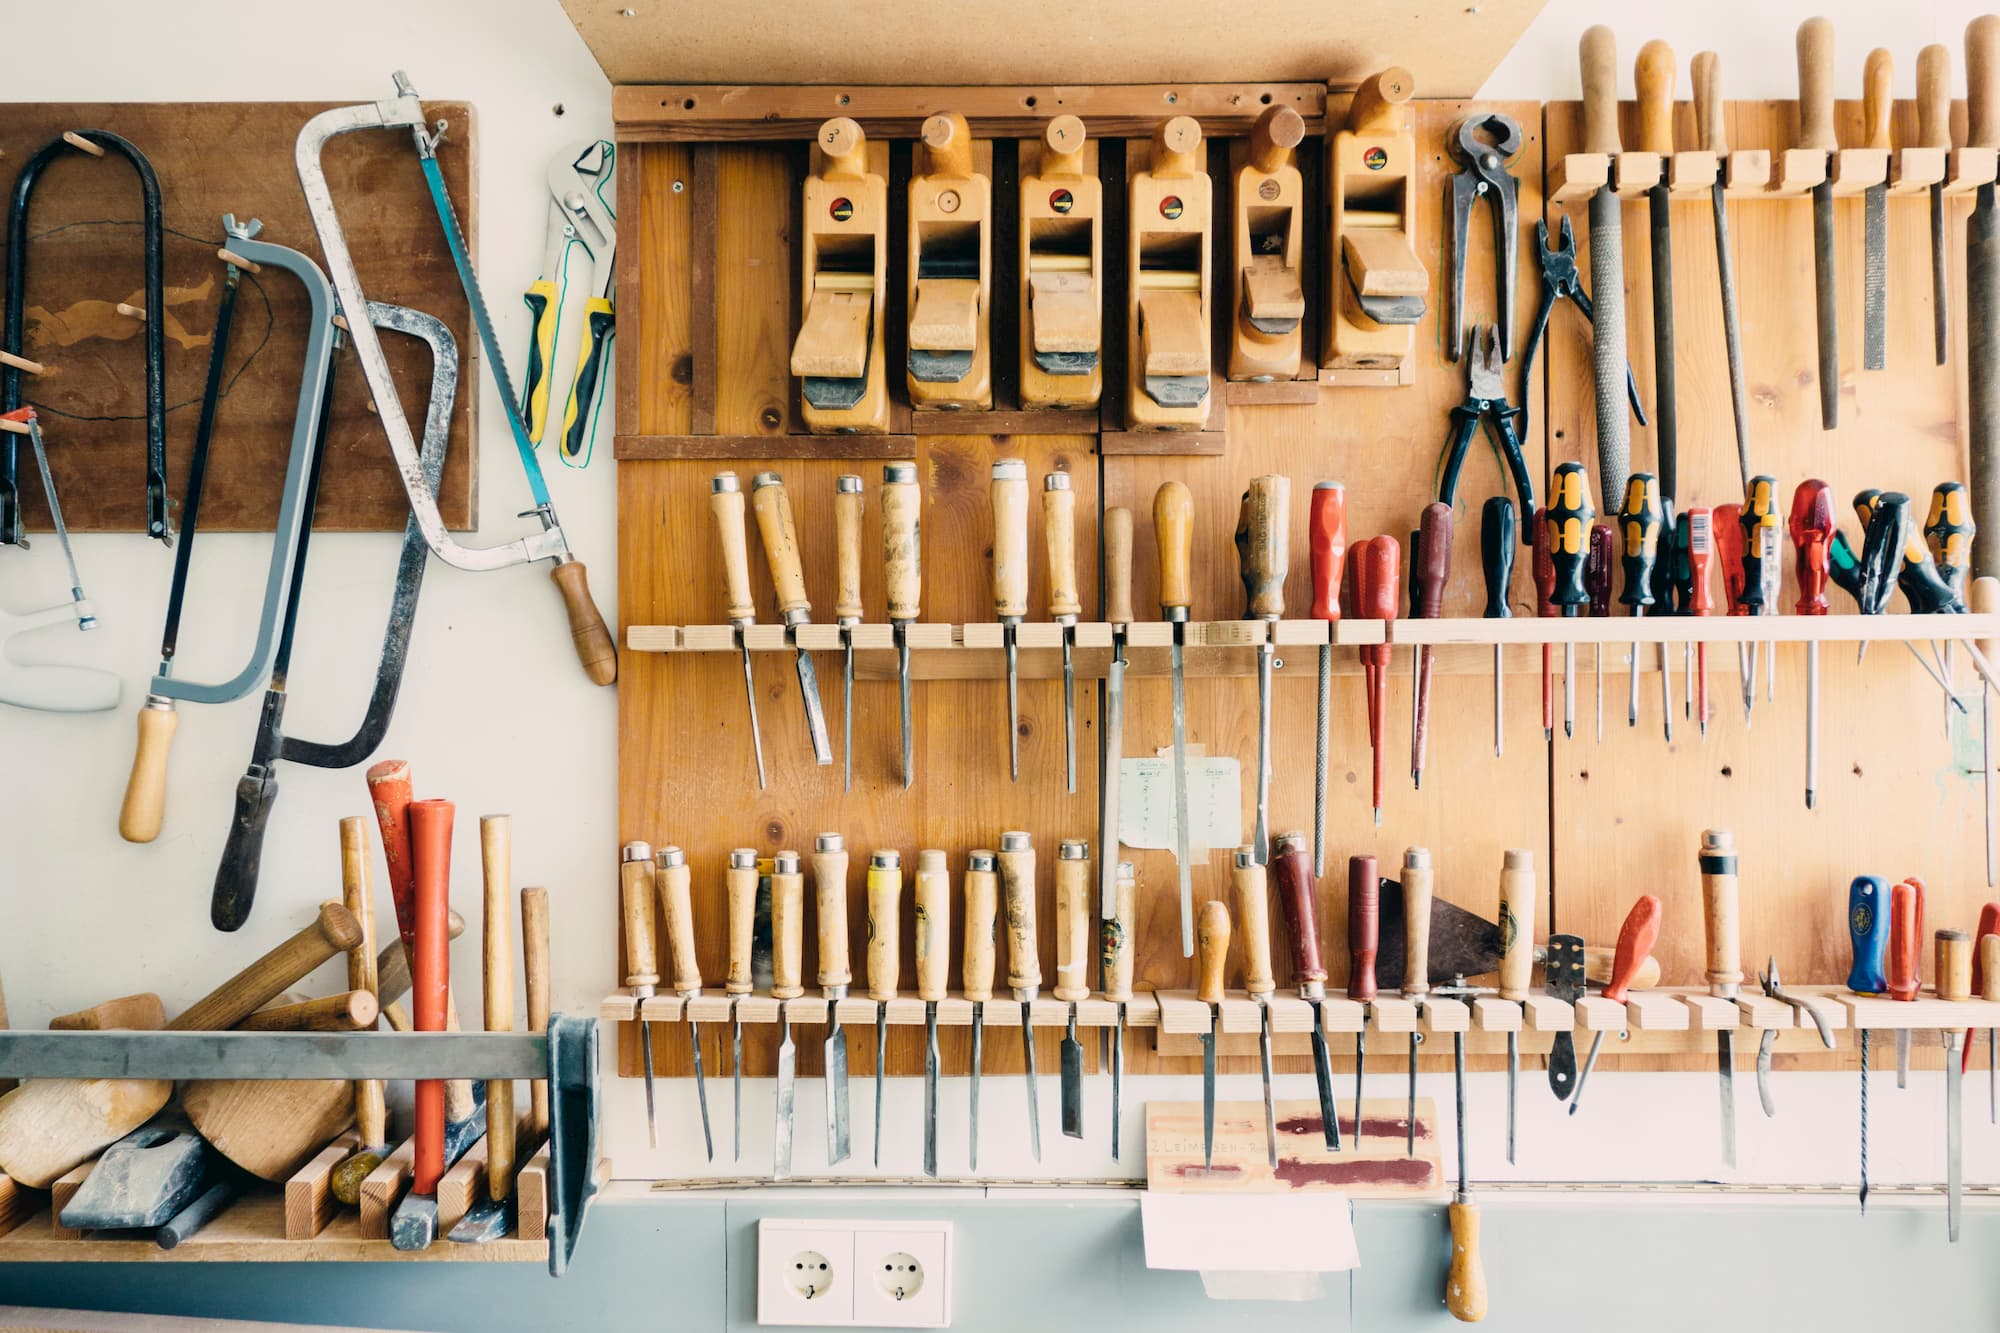
\includegraphics[width=1\linewidth]{fig/tool_set} \caption{Verschiedene Werkzeuge für unterschiedliche Aufgaben.}\label{fig:fig-werkzeuge}
\end{figure}

Die Tabelle unten listet wichtige Werkzeuge auf, die wir im weiteren Verlauf dieses Buches kennenlernen werden.

\begin{longtable}[]{@{}
  >{\raggedright\arraybackslash}p{(\columnwidth - 4\tabcolsep) * \real{0.04}}
  >{\raggedright\arraybackslash}p{(\columnwidth - 4\tabcolsep) * \real{0.37}}
  >{\raggedright\arraybackslash}p{(\columnwidth - 4\tabcolsep) * \real{0.59}}@{}}
\toprule
\begin{minipage}[b]{\linewidth}\raggedright
\textbf{Paket}
\end{minipage} & \begin{minipage}[b]{\linewidth}\raggedright
\textbf{Funktion}
\end{minipage} & \begin{minipage}[b]{\linewidth}\raggedright
\textbf{Aufgabe}
\end{minipage} \\
\midrule
\endhead
\texttt{tibble} & \texttt{as.tibble} & \href{14-daten-laden-und-sichten/tidyverse-und-tibbles.md}{Erstellt einen modernen Dataframe für tabellarische Daten}. \\
\texttt{readr} & \texttt{read\_csv} & \href{14-daten-laden-und-sichten/laden-eines-datensatzes.md}{Lesen von tabellarischen Datenformaten wie CSV-Dateien}. \\
\texttt{dplyr} & \texttt{select} & \href{15-daten-veraendern/spalten-auswaehlen.md}{Auswählen von Spalten (Variablen) eines Datensatzes}. \\
\texttt{dplyr} & \texttt{filter} & \href{15-daten-veraendern/zeilen-filtern.md}{Filtern von Daten auf Basis fast beliebiger Ausdrücke}. \\
\texttt{dplyr} & \texttt{mutate} & \href{15-daten-veraendern/spalten-veraendern/}{Hinzufügen neuer Spalten (Variablen)}. \\
\texttt{dplyr} & \texttt{recode} & \href{15-daten-veraendern/spalten-veraendern/spalten-neu-kodieren.md}{Spaltenwerte neu kodieren}. \\
\texttt{dplyr} & \texttt{arrange} & \href{15-daten-veraendern/zeilen-sortieren.md}{Die Reihenfolge von Zeilen verändern}. \\
\texttt{dplyr} & \texttt{group\_by} & \href{15-daten-veraendern/daten-zusammenfassen.md\#zusammenfassen-und-gruppieren}{Gruppieren von Daten}. \\
\texttt{dplyr} & \texttt{summarise} & \href{15-daten-veraendern/daten-zusammenfassen.md\#viele-zeilen-zu-einer-kennzahl-zusammenfassen}{Zusammenfassen von Daten}. \\
\texttt{ggplot2} & \texttt{ggplot}, \texttt{aes}, \texttt{geom\_line}\emph{,} \texttt{geom\_bar}, \texttt{geom\_col} \texttt{geom\_point} u.v.m. & \href{16-daten-visualisieren-mit-ggplot2/}{Visualisieren von Daten}. \\
\bottomrule
\end{longtable}

\hypertarget{das-paket-tibble}{%
\section{\texorpdfstring{Das Paket \texttt{tibble}}{Das Paket tibble}}\label{das-paket-tibble}}

Das Paket \texttt{tibble} führt das moderne Pendant zum klassischen Dataframe in R ein.

\begin{itemize}
\tightlist
\item
  \href{https://tibble.tidyverse.org/}{Zur offiziellen Webseite des \texttt{tibble} Pakets}
\end{itemize}

\hypertarget{das-paket-readr}{%
\section{\texorpdfstring{Das Paket \texttt{readr}}{Das Paket readr}}\label{das-paket-readr}}

Das Paket \texttt{readr} beinhaltet Funktionen für das Laden von Daten aus strukturierten Datenformaten wie CSV-Dateien. Alle Funktionen zum Datenimport aus readr erzeugen automatisch einen \texttt{tibble}.

\begin{itemize}
\tightlist
\item
  \href{https://readr.tidyverse.org/}{Zur offiziellen Webseite des \texttt{readr} Pakets}
\end{itemize}

\hypertarget{das-paket-dplyr}{%
\section{\texorpdfstring{Das Paket \texttt{dplyr}}{Das Paket dplyr}}\label{das-paket-dplyr}}

Das Paket \href{https://dplyr.tidyverse.org}{\texttt{dplyr}} hat einen etwas merkwürdigen Namen. Er setzt sich aus dem Buchstaben „d`` und dem abgekürzten Wort „plyr`` zusammen. Das „d`` steht für Dataframe, während „plyr`` für den englischen Begriff „plier`` steht, was auf Deutsch „Zange`` bedeutet. Passend dazu bildet das offizielle Symbol des Pakets mehrere Zangen ab.

\begin{itemize}
\tightlist
\item
  \href{https://dplyr.tidyverse.org/}{Zur offiziellen Dokumentation des \texttt{dplyr} Pakets}
\end{itemize}

\texttt{dplyr} liefert uns eine Vielzahl wichtiger Funktionen für die Manipulation von Daten, die in Form eines Tibble vorliegen. Eine Übersicht der Funktionen findet ihr in dem Cheat Sheet \href{https://raw.githubusercontent.com/rstudio/cheatsheets/main/data-transformation.pdf}{Data Transformation wit dplyr}.

\hypertarget{das-paket-ggplot2}{%
\section{\texorpdfstring{Das Paket \texttt{ggplot2}}{Das Paket ggplot2}}\label{das-paket-ggplot2}}

\texttt{ggplot2} ist eines der umfassendsten Pakete für die professionelle Visualisierung von Daten mit R:

\begin{itemize}
\tightlist
\item
  \href{https://ggplot2.tidyverse.org/}{Zur offiziellemn Dokumentation des \texttt{ggplot2} Pakets}
\end{itemize}

Das Cheat Sheet \href{https://raw.githubusercontent.com/rstudio/cheatsheets/main/data-visualization.pdf}{Data Visualization with ggplot2} beinhaltet alle wichtigen Funktionen im Überblick.

\hypertarget{part-explorative-datenanalyse-mit-r}{%
\part*{Explorative Datenanalyse mit R}\label{part-explorative-datenanalyse-mit-r}}
\addcontentsline{toc}{part}{Explorative Datenanalyse mit R}

\hypertarget{der-explorative-analyseprozess}{%
\chapter{Der explorative Analyseprozess}\label{der-explorative-analyseprozess}}

Dieser Abschnitt führt euch in die Grundlagen der \textbf{explorativen Datenanalyse} mit R ein. In der explorativen Datenanalyse versuchen wir einen unbekannten Datensatz mit geeigneten Verfahren kennenzulernen und schnell Muster in den Daten zu erkennen. Auf Basis dieser Muster formulieren wir \textbf{Hypothesen}. Diese Hypothesen können anschließend mit statistischen Modellen aus dem Bereich der schließenden Statistik auf ihre Gültigkeit überprüft werden. Die statistische Überprüfung ist jedoch nicht Teil der explorativen Datenanalyse nach dem Verständnis dieses Buches.

Eine ausgezeichnete Einführung in die explorative Datenanalyse mit R gibt auch das Buch \href{https://r4ds.had.co.nz}{R for Data Science} von \citet{wickham_r_2016}. Das Buch ist online frei zugänglich.

\begin{figure}

{\centering 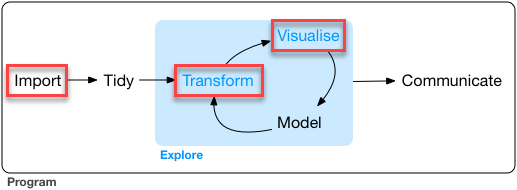
\includegraphics[width=0.6\linewidth]{fig/prozess_explorative_datenanalyse} 

}

\caption{Der Datenanalyseprozess.}\label{fig:der-explorative-analyse-prozess}
\end{figure}

\citet{wickham_r_2016} definieren den Datenanalyseprozess durch eine Abfolge bestimmter Schritte, wie in der Abbildung \ref{@der-explorative-analyse-prozess} gezeigt. In diesem Abschnitt stehen die rot markierten Schritte im Fokus.

\hypertarget{daten-laden}{%
\section{Daten laden}\label{daten-laden}}

Jeder Analyseprozess beginnt mit dem \href{}{Laden eines Datensatzes}. Dabei gibt es verschiedene Datenquellen, die in Betracht gezogen werden müssen. Ein häufig verwendetes Format sind Komma-separierte Werte (\textbf{C}omma \textbf{S}eparated \textbf{V}alues = CSV) in einfachen Textdateien. Dieses Format steht auch hier im Vordergrund.

Gemäß der Abbildung aus \citet{wickham_r_2016} folgt auf das Laden der Daten der Arbeitsschritt „Tidy``. Dieser ist dann notwendig, wenn die Daten nicht in der typischen Form bestehend aus Spalten und Zeilen vorliegen. Leider ist das in der Praxis oft der Fall. In diesem Buch wird aber zunächst davon ausgegangen, dass die Daten das entsprechende Format aufweisen. Die interessierte Leserin verweise ich auf das \href{https://r4ds.had.co.nz/tidy-data.html}{Kapitel 12 im Buch „R for Data Science``}.

\hypertarget{daten-transformieren}{%
\section{Daten transformieren}\label{daten-transformieren}}

Das Ziel der explorativen Datenanalyse ist die Visualisierung der Daten mit geeigneten Diagrammen, um interessante Muster sichtbar werden zu lassen. Visualisierungen benötigen häufig nur einen Teil der Daten (wenige Spalten oder bestimmte Zeilen). Auch müssen wir oft neue Spalten berechnen oder bestehende Daten aggregieren, bevor wir sie visualisieren können. Alle diese Aufgaben können wir unter dem Bereich der \textbf{Datentransformation} zusammenfassen.

Für diese Aufgaben bietet R mit dem Paket \texttt{dplyr} mächtige Funktionen. Insbesondere lernen wir in dem Abschnitt:

\begin{itemize}
\tightlist
\item
  Wie wir bestimmte Spalten auswählen können (dplyr-Verb: \texttt{select}).
\item
  Wie wir Zeilen fast beliebig filtern können (dplyr-Verb: \texttt{filter}).
\item
  Wie wir neue, berechnete Spalten hinzufügen können (dplyr-Verb: \texttt{mutate}).
\item
  Wie wir Zeilen sortieren können (dplyr-Verb: \texttt{arrange}).
\item
  Wie wir Zeilen zusammenfassen und gruppieren können (dplyr-Verben: \texttt{summarize} und \texttt{group\_by})
\end{itemize}

\hypertarget{daten-visualisieren}{%
\section{Daten visualisieren}\label{daten-visualisieren}}

Das wichtigste Werkzeug in der explorativen Datenanalyse ist die \textbf{Visualisierung von Daten}. In R steht uns dafür mit \texttt{ggplot2} ein leistungsfähiges Instrument zur Verfügung. Wir lernen für bestimmte Anwendungsfälle die richtigen Visualisierungen zu identifizieren und mit \texttt{ggplot2} umzusetzen.

\hypertarget{literatur}{%
\section{Literatur}\label{literatur}}

\hypertarget{buxfccher}{%
\subsection{Bücher}\label{buxfccher}}

Wickham, Hadley, and Garrett Grolemund. R for Data Science: Import, Tidy, Transform, Visualize, and Model Data. First edition, O'Reilly, 2016. Online verfügbar: \href{https://r4ds.had.co.nz}{https://r4ds.had.co.nz/}

Wickham, Hadley. ggplot2. Springer Science+Business Media, LLC, 2016. Online verfügbar: \href{https://ggplot2-book.org}{https://ggplot2-book.org/}

Kabacoff, Robert. R in Action: Data Analysis and Graphics with R. Second edition, Manning, 2015.

Sauer, Sebastian. Moderne Datenanalyse mit R: Daten einlesen, aufbereiten, visualisieren, modellieren und kommunizieren. Springer Gabler, 2019. Online verfügbar: \url{https://link.springer.com/book/10.1007/978-3-658-21587-3}

\hypertarget{online-dokumentationen}{%
\subsection{Online-Dokumentationen}\label{online-dokumentationen}}

\begin{itemize}
\tightlist
\item
  \href{https://www.tidyverse.org/}{Die offizielle Dokumentation der Tidyverse-Bibliotheken}
\item
  \href{https://ourcodingclub.github.io/tutorials/intro-to-r/}{Ein Tutorial für die Einführung in R mit RStudio}
\item
  \href{https://ourcodingclub.github.io/tutorials/data-manip-intro/}{Ein Tutorial zu den Grundlagen der Datenmanipulation mit R, \texttt{tidyr} und \texttt{dplyr}}
\item
  \href{https://ourcodingclub.github.io/tutorials/data-manip-efficient/}{Weiterführende Anleitungen zur Datenmanipulation mit \texttt{dplyr} (Efficient Data Manipulation)}
\item
  \href{https://ourcodingclub.github.io/tutorials/data-manip-creative-dplyr/}{Weiterführende Anleitungen zur Datenmanipulation mit \texttt{dplyr} (Advanced Data Manipulation)}
\end{itemize}

\hypertarget{spalten-auswuxe4hlen-mit-select}{%
\chapter{\texorpdfstring{Spalten auswählen mit \texttt{select}}{Spalten auswählen mit select}}\label{spalten-auswuxe4hlen-mit-select}}

\hypertarget{tldr-3}{%
\section*{TL;DR}\label{tldr-3}}

\begin{itemize}
\tightlist
\item
  Mit dem \texttt{select} Befehl können wir aus allen Spalten einer Tabelle eine Untermenge auswählen.
\item
  Neben einer Liste von gewünschten Spaltennamen können wir die Untermenge auch über den Ausschluss von nicht gewollten Spalten eingrenzen. Dafür verwenden wir das Zeichen \texttt{-} vor dem Spaltennamen.
\item
  Mit der Funktion \texttt{last\_col()} können wir die letzte oder die n-letzte Spalte auswählen
\item
  Mit dem Semikolon können wir Spaltenbereiche auswählen und so beispielsweise alle Spalten von der 5. bis zur vorletzten selektieren (\texttt{select(5\ :\ last\_col(2))}).
\item
  Wir können Spalten anhand ihres Datentyps selektieren (\texttt{is.numeric}, \texttt{is.character}, etc.).
\item
  Wir können Spalten über die Zugehörigkeit zu einer Liste selektieren (\texttt{all\_of}, \texttt{any\_of}).
\end{itemize}

\hypertarget{beispieldaten-pokuxe9mon}{%
\section{Beispieldaten: Pokémon}\label{beispieldaten-pokuxe9mon}}

Es ist ratsam die verfügbaren Spalten eines Datensatzes zu kennen, bevor wir uns mit einigen Beispielen beschäftigen, wie wir Bestimmte davon auswählen können. Für dieses Kapitel verwenden wir den \href{https://www.kaggle.com/rounakbanik/pokemon/version/1}{Pokémon-Datensatz}, der auf \href{https://kaggle.com/}{Kaggle.com} bereitgestellt wird.

\begin{Shaded}
\begin{Highlighting}[]
\NormalTok{pokemon }\OtherTok{\textless{}{-}} \FunctionTok{read\_csv}\NormalTok{(}\StringTok{"datasets/pokemon.csv"}\NormalTok{)}
\end{Highlighting}
\end{Shaded}

Nach dem Laden des Datensatzes lassen wir uns mit \texttt{colnames()} die Spalten anzeigen:

\begin{Shaded}
\begin{Highlighting}[]
\NormalTok{pokemon }\SpecialCharTok{\%\textgreater{}\%} \FunctionTok{colnames}\NormalTok{()}
\end{Highlighting}
\end{Shaded}

\begin{verbatim}
##  [1] "abilities"         "against_bug"       "against_dark"     
##  [4] "against_dragon"    "against_electric"  "against_fairy"    
##  [7] "against_fight"     "against_fire"      "against_flying"   
## [10] "against_ghost"     "against_grass"     "against_ground"   
## [13] "against_ice"       "against_normal"    "against_poison"   
## [16] "against_psychic"   "against_rock"      "against_steel"    
## [19] "against_water"     "attack"            "base_egg_steps"   
## [22] "base_happiness"    "base_total"        "capture_rate"     
## [25] "classfication"     "defense"           "experience_growth"
## [28] "height_m"          "hp"                "japanese_name"    
## [31] "name"              "percentage_male"   "pokedex_number"   
## [34] "sp_attack"         "sp_defense"        "speed"            
## [37] "type1"             "type2"             "weight_kg"        
## [40] "generation"        "is_legendary"
\end{verbatim}

Das sind mehr als 40 Spalten. Wie viele genau?

\begin{Shaded}
\begin{Highlighting}[]
\NormalTok{pokemon }\SpecialCharTok{\%\textgreater{}\%} \FunctionTok{dim}\NormalTok{()}
\end{Highlighting}
\end{Shaded}

\begin{verbatim}
## [1] 801  41
\end{verbatim}

Oder mit \texttt{ncol()}:

\begin{Shaded}
\begin{Highlighting}[]
\NormalTok{pokemon }\SpecialCharTok{\%\textgreater{}\%} \FunctionTok{ncol}\NormalTok{()}
\end{Highlighting}
\end{Shaded}

\begin{verbatim}
## [1] 41
\end{verbatim}

Es sind also 41 Spalten. Genug um die wichtigsten Funktionen für das Auswählen von Spalten zu zeigen.

\hypertarget{bestimmte-spalten-nach-namen-auswuxe4hlen}{%
\section{Bestimmte Spalten nach Namen auswählen}\label{bestimmte-spalten-nach-namen-auswuxe4hlen}}

Die Funktion \texttt{select} verwenden wir für das Auswählen einer Untermenge an Spalten. Wir können im einfachsten Fall einfach die gewünschten Spalten mit Kommata getrennt auflisten:

\begin{Shaded}
\begin{Highlighting}[]
\NormalTok{pokemon }\SpecialCharTok{\%\textgreater{}\%}
  \FunctionTok{select}\NormalTok{(name, type1)}
\end{Highlighting}
\end{Shaded}

\begin{verbatim}
## # A tibble: 801 x 2
##    name       type1
##    <chr>      <chr>
##  1 Bulbasaur  grass
##  2 Ivysaur    grass
##  3 Venusaur   grass
##  4 Charmander fire 
##  5 Charmeleon fire 
##  6 Charizard  fire 
##  7 Squirtle   water
##  8 Wartortle  water
##  9 Blastoise  water
## 10 Caterpie   bug  
## # ... with 791 more rows
\end{verbatim}

Dabei können wir beliebig viele Spalten in die Liste aufnehmen:

\begin{Shaded}
\begin{Highlighting}[]
\NormalTok{pokemon }\SpecialCharTok{\%\textgreater{}\%}
  \FunctionTok{select}\NormalTok{(name, type1, type2, is\_legendary)}
\end{Highlighting}
\end{Shaded}

\begin{verbatim}
## # A tibble: 801 x 4
##    name       type1 type2  is_legendary
##    <chr>      <chr> <chr>         <dbl>
##  1 Bulbasaur  grass poison            0
##  2 Ivysaur    grass poison            0
##  3 Venusaur   grass poison            0
##  4 Charmander fire  <NA>              0
##  5 Charmeleon fire  <NA>              0
##  6 Charizard  fire  flying            0
##  7 Squirtle   water <NA>              0
##  8 Wartortle  water <NA>              0
##  9 Blastoise  water <NA>              0
## 10 Caterpie   bug   <NA>              0
## # ... with 791 more rows
\end{verbatim}

\hypertarget{minus-operator}{%
\section{Spalten aus der Auswahl ausschließen}\label{minus-operator}}

Wollen wir fast alle verfügbaren Spalten auswählen, so ist es effizienter, die Spalten zu nennen, die wir ausschließen wollen. Das können wir mit dem Minus-Symbol erreichen:

\begin{Shaded}
\begin{Highlighting}[]
\NormalTok{pokemon }\SpecialCharTok{\%\textgreater{}\%}
  \FunctionTok{select}\NormalTok{(}\SpecialCharTok{{-}}\NormalTok{is\_legendary)}
\end{Highlighting}
\end{Shaded}

\hypertarget{die-letzte-oder-n-letzten-spalten-auswuxe4hlen}{%
\section{Die letzte oder n-letzten Spalten auswählen}\label{die-letzte-oder-n-letzten-spalten-auswuxe4hlen}}

\begin{Shaded}
\begin{Highlighting}[]
\NormalTok{pokemon }\SpecialCharTok{\%\textgreater{}\%}
  \FunctionTok{select}\NormalTok{(}\FunctionTok{last\_col}\NormalTok{())}
\end{Highlighting}
\end{Shaded}

\begin{verbatim}
## # A tibble: 801 x 1
##    is_legendary
##           <dbl>
##  1            0
##  2            0
##  3            0
##  4            0
##  5            0
##  6            0
##  7            0
##  8            0
##  9            0
## 10            0
## # ... with 791 more rows
\end{verbatim}

\hypertarget{spalten-nach-datentyp-selektieren}{%
\section{Spalten nach Datentyp selektieren}\label{spalten-nach-datentyp-selektieren}}

Manchmal möchten wir Spalten nach ihrem Datentyp auswählen. Für die Prüfung, ob eine Spalte oder ein Wert einem bestimmten Datentyp entspricht, gibt es Funktionen in R:

\begin{itemize}
\tightlist
\item
  \texttt{is.numeric} prüft, ob eine Spalte oder ein Wert numerisch ist.
\item
  \texttt{is.character} prüft, ob es sich um eine alphanumerische Spalte handelt (Zeichenketten oder Strings).
\item
  \texttt{is.logical} prüft, ob es sich um eine Spalte mit Wahrheitswerten handelt (Bool'scher Datentyp).
\item
  \texttt{is.factor} prüft, ob es sich bei einer Spalte um einen Faktor mit einer fest definierten Anzahl von Ausprägungen handelt.
\end{itemize}

Um beispielsweise alle numersichen Spalten im Pokémon-Datensatz auszuwählen, können wir den folgenden Aufruf verwenden:

\begin{Shaded}
\begin{Highlighting}[]
\NormalTok{pokemon }\SpecialCharTok{\%\textgreater{}\%} 
  \FunctionTok{select}\NormalTok{(}\FunctionTok{where}\NormalTok{(is.numeric))}
\end{Highlighting}
\end{Shaded}

\begin{verbatim}
## # A tibble: 801 x 34
##    against_bug against_dark against_dragon against_electric against_fairy
##          <dbl>        <dbl>          <dbl>            <dbl>         <dbl>
##  1        1               1              1              0.5           0.5
##  2        1               1              1              0.5           0.5
##  3        1               1              1              0.5           0.5
##  4        0.5             1              1              1             0.5
##  5        0.5             1              1              1             0.5
##  6        0.25            1              1              2             0.5
##  7        1               1              1              2             1  
##  8        1               1              1              2             1  
##  9        1               1              1              2             1  
## 10        1               1              1              1             1  
## # ... with 791 more rows, and 29 more variables: against_fight <dbl>,
## #   against_fire <dbl>, against_flying <dbl>, against_ghost <dbl>,
## #   against_grass <dbl>, against_ground <dbl>, against_ice <dbl>,
## #   against_normal <dbl>, against_poison <dbl>, against_psychic <dbl>,
## #   against_rock <dbl>, against_steel <dbl>, against_water <dbl>, attack <dbl>,
## #   base_egg_steps <dbl>, base_happiness <dbl>, base_total <dbl>,
## #   defense <dbl>, experience_growth <dbl>, height_m <dbl>, hp <dbl>, ...
\end{verbatim}

Der \texttt{where} Funktion können wir eine Funktion übergeben, die in Bezug auf eine Spalte wahr oder falsch zurückliefert.

Leider existiert keine Standardfunktion, um Spalten auf den Datentyp \texttt{date} zu prüfen. Wir können uns diese aber einfach selbst schreiben:

\begin{Shaded}
\begin{Highlighting}[]
\CommentTok{\# Funktion, um Datumsspalten zu erkennen}
\NormalTok{is.date }\OtherTok{\textless{}{-}} \ControlFlowTok{function}\NormalTok{(x) \{}
  \FunctionTok{inherits}\NormalTok{(x, }\FunctionTok{c}\NormalTok{(}\StringTok{"Date"}\NormalTok{, }\StringTok{"POSIXt"}\NormalTok{))}
\NormalTok{\}}

\NormalTok{pokemon }\SpecialCharTok{\%\textgreater{}\%} 
  \FunctionTok{select}\NormalTok{(}\FunctionTok{where}\NormalTok{(is.date))}
\end{Highlighting}
\end{Shaded}

\begin{verbatim}
## # A tibble: 801 x 0
\end{verbatim}

Für den Pokémon-Datensatz ist das Ergebnis leer, das heißt es existiert keine Spalte vom Typ Datum.

\hypertarget{spaltenmengen-definieren-und-selektieren}{%
\section{Spaltenmengen definieren und selektieren}\label{spaltenmengen-definieren-und-selektieren}}

Häufig benötigt man in unterschiedlichen Abfragen die gleichen Spalten. Um nicht jedes Mal die gesamte Liste aufführen zu müssen, können wir in diesem Fall einen Vektor definieren, der die Namen der Spalten enthält. Mit der \texttt{all\_of} Funktion können wir dann alle Spalten in diesem Vektor auswählen:

\begin{Shaded}
\begin{Highlighting}[]
\CommentTok{\# Erstellen eines Vektors mit gewünschten Spaltennamen}
\NormalTok{vars }\OtherTok{\textless{}{-}} \FunctionTok{c}\NormalTok{(}\StringTok{"name"}\NormalTok{, }\StringTok{"type1"}\NormalTok{, }\StringTok{"type2"}\NormalTok{)}

\CommentTok{\# Selektieren auf Basis dieser Menge}
\NormalTok{pokemon }\SpecialCharTok{\%\textgreater{}\%}
  \FunctionTok{select}\NormalTok{(}\FunctionTok{all\_of}\NormalTok{(vars))}
\end{Highlighting}
\end{Shaded}

\begin{verbatim}
## # A tibble: 801 x 3
##    name       type1 type2 
##    <chr>      <chr> <chr> 
##  1 Bulbasaur  grass poison
##  2 Ivysaur    grass poison
##  3 Venusaur   grass poison
##  4 Charmander fire  <NA>  
##  5 Charmeleon fire  <NA>  
...
\end{verbatim}

Wir können bei Bedarf auch einzelne Elemente der Menge über den \protect\hyperlink{minus-operator}{Minus-Operator} ausschließen:

\begin{Shaded}
\begin{Highlighting}[]
\CommentTok{\# Selektieren auf Basis dieser Menge, aber ohne "type2"}
\NormalTok{pokemon }\SpecialCharTok{\%\textgreater{}\%} 
  \FunctionTok{select}\NormalTok{(}\FunctionTok{all\_of}\NormalTok{(vars), }\SpecialCharTok{{-}}\NormalTok{type2)}
\end{Highlighting}
\end{Shaded}

\begin{verbatim}
## # A tibble: 801 x 2
##    name       type1
##    <chr>      <chr>
##  1 Bulbasaur  grass
##  2 Ivysaur    grass
##  3 Venusaur   grass
##  4 Charmander fire 
##  5 Charmeleon fire 
...
\end{verbatim}

Mit \texttt{any\_of} können wir auch Spalten im Vektor aufnehmen, die nicht existieren. Es werden dann alle Spalten selektiert, die in der Liste vorkommen und auch tatsächlich im Tibble vorhanden sind. So können wir einen Vektor erstellen, der Spaltennamen aus unterschiedlichen Datensätzen beinhaltet:

\begin{Shaded}
\begin{Highlighting}[]
\CommentTok{\# Erstellen eines Vektors mit gewünschten Spaltennamen, "type3" existiert nicht im Tibble}
\NormalTok{vars }\OtherTok{\textless{}{-}} \FunctionTok{c}\NormalTok{(}\StringTok{"name"}\NormalTok{, }\StringTok{"type1"}\NormalTok{, }\StringTok{"type2"}\NormalTok{, }\StringTok{"type3"}\NormalTok{)}

\CommentTok{\# Selektieren auf Basis dieser Menge, "type3" ist jedoch nicht vorhanden}
\NormalTok{pokemon }\SpecialCharTok{\%\textgreater{}\%}
  \FunctionTok{select}\NormalTok{(}\FunctionTok{any\_of}\NormalTok{(vars))}
\end{Highlighting}
\end{Shaded}

\begin{verbatim}
## # A tibble: 801 x 3
##    name       type1 type2 
##    <chr>      <chr> <chr> 
##  1 Bulbasaur  grass poison
##  2 Ivysaur    grass poison
##  3 Venusaur   grass poison
##  4 Charmander fire  <NA>  
##  5 Charmeleon fire  <NA>  
...
\end{verbatim}

\hypertarget{weitere-online-quellen}{%
\section{Weitere Online-Quellen}\label{weitere-online-quellen}}

\begin{itemize}
\tightlist
\item
  \href{https://dplyr.tidyverse.org/reference/select.html}{Offizielle Dokumentation des \texttt{select} Befehls im Tidyverse}.
\item
  \href{https://r4ds.had.co.nz/transform.html\#select}{Kapitel 5.4} aus \citet{wickham_r_2016}
\end{itemize}

\hypertarget{zeilen-filtern-mit-filter}{%
\chapter{\texorpdfstring{Zeilen filtern mit \texttt{filter}}{Zeilen filtern mit filter}}\label{zeilen-filtern-mit-filter}}

\hypertarget{tldr-4}{%
\section*{TL;DR}\label{tldr-4}}

\begin{itemize}
\tightlist
\item
  Mit dem \texttt{filter} Befehl können wir eine Untermenge der gesamten Zeilen eines Datensatzes auswählen.
\item
  Alphanumersiche nominalskalierte Spalten können wir mit dem \texttt{==} Operator auf einen bestimmten Wert filtern.
\end{itemize}

\hypertarget{filtern-von-alphanumerischen-werten-zeichenketten}{%
\section{Filtern von alphanumerischen Werten (Zeichenketten)}\label{filtern-von-alphanumerischen-werten-zeichenketten}}

\hypertarget{filtern-auf-gleichheit}{%
\subsection{Filtern auf Gleichheit}\label{filtern-auf-gleichheit}}

\begin{Shaded}
\begin{Highlighting}[]
\NormalTok{pokemon }\SpecialCharTok{\%\textgreater{}\%}
  \FunctionTok{select}\NormalTok{(name, type1) }\SpecialCharTok{\%\textgreater{}\%}
  \FunctionTok{filter}\NormalTok{(type1 }\SpecialCharTok{==} \StringTok{"electric"}\NormalTok{)}
\end{Highlighting}
\end{Shaded}

\begin{verbatim}
## # A tibble: 39 x 2
##    name       type1   
##    <chr>      <chr>   
##  1 Pikachu    electric
##  2 Raichu     electric
##  3 Magnemite  electric
##  4 Magneton   electric
##  5 Voltorb    electric
...
\end{verbatim}

\hypertarget{filtern-uxfcber-eine-liste-von-werten}{%
\subsection{Filtern über eine Liste von Werten}\label{filtern-uxfcber-eine-liste-von-werten}}

\begin{Shaded}
\begin{Highlighting}[]
\NormalTok{pokemon }\SpecialCharTok{\%\textgreater{}\%}
  \FunctionTok{select}\NormalTok{(name, type1) }\SpecialCharTok{\%\textgreater{}\%}
  \FunctionTok{filter}\NormalTok{(type1 }\SpecialCharTok{\%in\%} \FunctionTok{c}\NormalTok{(}\StringTok{"electric"}\NormalTok{, }\StringTok{"poison"}\NormalTok{, }\StringTok{"fire"}\NormalTok{))}
\end{Highlighting}
\end{Shaded}

\begin{verbatim}
## # A tibble: 123 x 2
##    name       type1   
##    <chr>      <chr>   
##  1 Charmander fire    
##  2 Charmeleon fire    
##  3 Charizard  fire    
##  4 Ekans      poison  
##  5 Arbok      poison  
##  6 Pikachu    electric
...
\end{verbatim}

Wenn wir die Liste im mehreren Operationen wiederverwenden wollen, können wir sie auch einmal auf einer Variable speichern und in der \texttt{filter} Funktion darauf zugreifen:

\begin{Shaded}
\begin{Highlighting}[]
\NormalTok{search\_types }\OtherTok{\textless{}{-}} \FunctionTok{c}\NormalTok{(}\StringTok{"electric"}\NormalTok{, }\StringTok{"poison"}\NormalTok{, }\StringTok{"fire"}\NormalTok{)}

\NormalTok{pokemon }\SpecialCharTok{\%\textgreater{}\%}
  \FunctionTok{select}\NormalTok{(name, type1) }\SpecialCharTok{\%\textgreater{}\%}
  \FunctionTok{filter}\NormalTok{(type1 }\SpecialCharTok{\%in\%}\NormalTok{ search\_types)}
\end{Highlighting}
\end{Shaded}

\begin{verbatim}
## # A tibble: 123 x 2
##    name       type1   
##    <chr>      <chr>   
##  1 Charmander fire    
##  2 Charmeleon fire    
##  3 Charizard  fire    
##  4 Ekans      poison  
##  5 Arbok      poison  
...
\end{verbatim}

\hypertarget{suchen-nach-dem-vorkommen-eines-wertes-in-einem-string}{%
\subsection{Suchen nach dem Vorkommen eines Wertes in einem String}\label{suchen-nach-dem-vorkommen-eines-wertes-in-einem-string}}

Um einen String auf das Vorhandensein eines bestimmten Wertes zu durchsuchen können wir auf die \texttt{str\_detect} Funktion aus dem \texttt{stringr} Paket zurückgreifen. \texttt{stringr} ist ebenfalls im Tidyverse enthalten:

\begin{Shaded}
\begin{Highlighting}[]
\NormalTok{pokemon }\SpecialCharTok{\%\textgreater{}\%}
  \FunctionTok{select}\NormalTok{(name) }\SpecialCharTok{\%\textgreater{}\%}
  \FunctionTok{filter}\NormalTok{(}\FunctionTok{str\_detect}\NormalTok{(name, }\StringTok{"chu"}\NormalTok{))}
\end{Highlighting}
\end{Shaded}

\begin{verbatim}
## # A tibble: 4 x 1
##   name    
##   <chr>   
## 1 Pikachu 
## 2 Raichu  
## 3 Pichu   
## 4 Smoochum
\end{verbatim}

\hypertarget{suchen-nach-mustern-in-einem-string}{%
\subsection{Suchen nach Mustern in einem String}\label{suchen-nach-mustern-in-einem-string}}

Wir können auch nach Mustern suchen, ähnlich was der SQL-Befehl \texttt{like} erlaubt:

\begin{Shaded}
\begin{Highlighting}[]
\FunctionTok{library}\NormalTok{(stringr)}
\NormalTok{pokemon }\SpecialCharTok{\%\textgreater{}\%}
  \FunctionTok{select}\NormalTok{(name) }\SpecialCharTok{\%\textgreater{}\%}
  \FunctionTok{filter}\NormalTok{(}\FunctionTok{str\_like}\NormalTok{(name, }\StringTok{\textquotesingle{}\%chu\textquotesingle{}}\NormalTok{))}
\end{Highlighting}
\end{Shaded}

\begin{verbatim}
## # A tibble: 3 x 1
##   name   
##   <chr>  
## 1 Pikachu
## 2 Raichu 
## 3 Pichu
\end{verbatim}

\hypertarget{part-fallstudien}{%
\part*{Fallstudien}\label{part-fallstudien}}
\addcontentsline{toc}{part}{Fallstudien}

\hypertarget{fallstudie-orangenlimonade}{%
\chapter{Fallstudie Orangenlimonade}\label{fallstudie-orangenlimonade}}

\hypertarget{einfuxfchrung}{%
\section{Einführung}\label{einfuxfchrung}}

\begin{Shaded}
\begin{Highlighting}[]
\NormalTok{limo }\OtherTok{\textless{}{-}} \FunctionTok{read\_csv}\NormalTok{(}\StringTok{"datasets/limonade.csv"}\NormalTok{)}
\end{Highlighting}
\end{Shaded}

\begin{Shaded}
\begin{Highlighting}[]
\NormalTok{limo }\SpecialCharTok{\%\textgreater{}\%} 
  \FunctionTok{select}\NormalTok{(f44\_studiengang) }\SpecialCharTok{\%\textgreater{}\%} 
  \FunctionTok{head}\NormalTok{() }\SpecialCharTok{\%\textgreater{}\%} 
  \FunctionTok{kable}\NormalTok{()}
\end{Highlighting}
\end{Shaded}

\begin{tabular}{r}
\hline
f44\_studiengang\\
\hline
1\\
\hline
1\\
\hline
1\\
\hline
2\\
\hline
2\\
\hline
2\\
\hline
\end{tabular}

\begin{Shaded}
\begin{Highlighting}[]
\NormalTok{limo }\SpecialCharTok{\%\textgreater{}\%} \FunctionTok{colnames}\NormalTok{()}
\end{Highlighting}
\end{Shaded}

\begin{verbatim}
##   [1] "id"                                 "f1_gekauft"                        
##   [3] "f1_getrunken"                       "f1_weder_noch"                     
##   [5] "f2_grund_nichtkauf"                 "f3_discounter"                     
##   [7] "f3_getraenkemarkt"                  "f3_kaufhaus"                       
##   [9] "f3_kiosk"                           "f3_sonstige"                       
##  [11] "f3_supermarkt"                      "f4_konsumhaeufigkeit"              
##  [13] "f5_flaschenzahl_025_AB"             "f5_flaschenzahl_033_AB"            
##  [15] "f5_flaschenzahl_050_AB"             "f5_flaschenzahl_075_AB"            
...
\end{verbatim}

\hypertarget{part-anhang}{%
\part*{Anhang}\label{part-anhang}}
\addcontentsline{toc}{part}{Anhang}

\hypertarget{datensaetze}{%
\chapter*{Datensätze}\label{datensaetze}}
\addcontentsline{toc}{chapter}{Datensätze}

\begin{longtable}[]{@{}
  >{\raggedright\arraybackslash}p{(\columnwidth - 4\tabcolsep) * \real{0.51}}
  >{\raggedright\arraybackslash}p{(\columnwidth - 4\tabcolsep) * \real{0.33}}
  >{\raggedright\arraybackslash}p{(\columnwidth - 4\tabcolsep) * \real{0.15}}@{}}
\caption{Datensätze in diesem Buch}\tabularnewline
\toprule
\endhead
\textbf{Name} & \textbf{Download-Link} & \textbf{Kategorie} \\
Online-Umfrage zum Kaufverhalten von Orangenlimonade & \href{datasets/limonade.csv}{Download} & Marktforschung \\
Tweets ausgewählter deutscher Politiker:innen & Download & Soziale Medien \\
Pokémon & \href{datasets/pokemon.csv}{Download} & TV \\
\bottomrule
\end{longtable}

  \bibliography{book.bib,packages.bib}

\end{document}
